\problemname{Alternative Architecture}

\begin{wrapfigure}{r}{0.3\textwidth}
  \vspace{-5mm}
  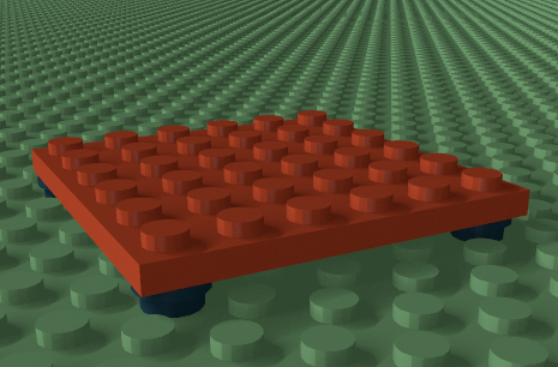
\includegraphics[width=0.3\textwidth]{rotated-plate.png}
  \caption{Placing a $6\times6$ plate diagonally.}
  \vspace{-5mm}
  \label{fig:rotated}
\end{wrapfigure}
In his free time, Thomas greatly enjoys working on the extensive Lego project
that he has built in his attic, adding house after house to his miniature city.
However, he has become a bit bored with the completely rectangular layout that
is enforced by the little studs of the huge base plate that his city is built
on.

After an exchange with some other Lego creators he came across a technique that
will allow him to place his buildings at different angles. Each building rests
on a rectangular ground plate, to the underside of which he attaches four round
$1\times 1$-plates in the corners. These $1\times 1$-plates are then placed on
four studs of the base plate, like in Figure~\ref{fig:rotated}.

If the ground plate of the building is $a\times b$ studs, what is the number of
orientations it can be placed in using this technique, so that all the corner
plates exactly fit on studs of the base plate?

\begin{figure}[!h]
  \centering
  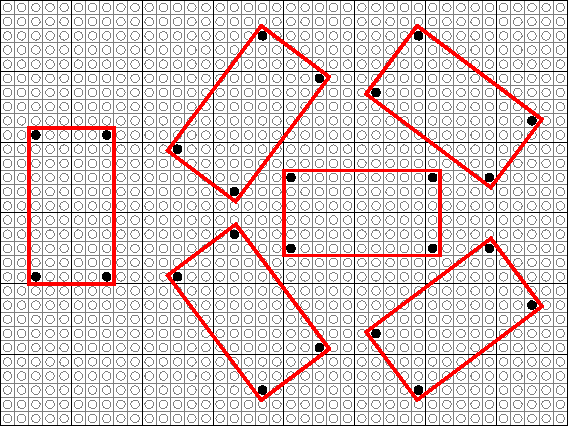
\includegraphics[width=0.6\textwidth]{sample2}
  \caption{Illustration of the first sample case. There are many ways of
  placing a $6 \times 11$ plate, but only $6$ distinct orientations.}
\end{figure}

\begin{Input}
  The input consists of:
  \begin{itemize}
    \item One line with two integers $a$ and $b$ ($2 \le a,b \le 10^6$), the
		dimensions of the ground plate the building is resting on.
  \end{itemize}
\end{Input}

\begin{Output}
  Output one integer, the number of different orientations the ground plate can
  be placed in.
\end{Output}
